\documentclass[12pt,a4paper]{article}

% Pacotes básicos
\usepackage[utf8]{inputenc}     % Codificação do arquivo
\usepackage[T1]{fontenc}        % Acentos corretos
\usepackage[brazil]{babel}      % Português do Brasil
\usepackage{graphicx}           % Inclusão de imagens
\usepackage{float}              % Melhor controle de posição de figuras/tabelas
\usepackage{amsmath, amssymb}   % Símbolos matemáticos
\usepackage{hyperref}           % Links clicáveis
\usepackage{caption}            % Legendas personalizadas
\usepackage{cite}               % Gerenciamento de citações
\usepackage{listings}           % para formatar blocos de código
\usepackage{enumitem}           % para controlar listas
\usepackage{xcolor}             % necessário para cores no listings

% Configurações do listings
\lstset{
  language=Python,
  basicstyle=\ttfamily\small,
  numbers=left,
  numberstyle=\tiny,
  frame=single,
  breaklines=true,
  keywordstyle=\color{blue}\bfseries,
  stringstyle=\color{red},
  commentstyle=\color{green!60!black}\itshape,
  showstringspaces=false
}

\graphicspath{{./img/}} % Diretório das imagens

\begin{document}

% ==============================
% CAPA
% ==============================
\begin{titlepage}
    \centering
    {\Large \textbf{Universidade Federal de Minas Gerais}}\\[0.3cm]
    {\large Engenharia de Sistemas}\\[2cm]
    
    {\Huge \textbf{Relatório do Trabalho Prático II - Coloração em Grafos}}\\[1.5cm]
    
    \textbf{Fundamentos de Inteligência Artificial}\\[0.5cm]
    \textbf{Professores:} Cristiano Castro e João Pedro Campos\\[1.5cm]
    
    \begin{flushleft}
        \textbf{Alunos:}\\
        Áquila Oliveira Souza --- 2021019327\\
        Arthur Jorge --- 2022055718\\
        Felippe Veloso Marinho --- 2021072260\\
        Jefferson Pereira de Souza --- 2022099049\\
        Josoé Santos Queiroz --- 2019026982
    \end{flushleft}
    
    \vfill
    {\large Belo Horizonte, MG}\\
    {\large \today}
\end{titlepage}

\clearpage
\tableofcontents
\clearpage

% ==============================
% INTRODUÇÃO
% ==============================
\section{Introdução}
A coloração de grafos é um problema clássico da teoria dos grafos com diversas aplicações práticas, como na alocação de frequências em redes sem fio, escalonamento de tarefas e planejamento de horários. O objetivo é atribuir cores aos vértices de um grafo de forma que vértices adjacentes não compartilhem a mesma cor, minimizando o número total de cores utilizadas.

Neste relatório, apresentamos uma solução para o problema de coloração de grafos, modelando-o formalmente como um grafo em que as arestas representam restrições binárias entre os vértices. 

Além disso, detalhamos as heurísticas utilizadas para resolver o problema, discutindo suas abordagens teóricas e implementações práticas. Também analisamos as decisões tomadas durante o desenvolvimento e os resultados obtidos.

O documento está organizado da seguinte forma: na Seção 2, apresentamos o problema de coloração de grafos; na Seção 3, discutimos as heurísticas teóricas; na Seção 4, detalhamos suas implementações; e, por fim, na Seção 5, apresentamos as conclusões e possíveis melhorias futuras.
\section{Problema da coloração em grafos}

\section{Heurísticas - Teoria}
Nessa sessão será definido como cada uma das heurísticas são.

\subsection{Random Walk (RW)}
O Random Walk é uma heurística de busca estocástica que explora o espaço de soluções movendo-se aleatoriamente entre as distribuições do grafo para encontrar uma coloração viável. 

A ideia principal é começar com uma coloração inicial (geralmente aleatória) e, em seguida, ajustar os conflitos, ou seja, resolver os casos em que vértices adjacentes possuem a mesma cor. Esse processo é repetido até que uma solução aceitável seja encontrada ou até que um critério de parada seja atingido.

\subsection{Best Improvement (BI)}
O Best Improvement é uma heurística que busca a melhor solução possível em cada iteração. O Best Improvement (BI) é uma heurística de busca local usada para melhorar uma solução já existente. 

A ideia é que, inicialmente, temos uma solução e, a partir dela, buscamos melhorá-la realizando pequenas alterações. Em vez de aceitar a primeira melhoria encontrada, o BI verifica todas as possíveis mudanças e escolhe aquela que oferece o maior benefício.

No contexto do problema de coloração de grafos, o objetivo é minimizar o número de conflitos (quando vértices vizinhos possuem a mesma cor) ou reduzir a quantidade de cores utilizadas para resolver o problema.

\subsection{First Improvement with Random Local Search (FI-RS)}

O algoritmo segue uma abordagem estocástica para atribuição de cores às variáveis. Inicialmente, uma variável é escolhida de forma aleatória. Em seguida, seleciona-se uma cor aleatória para essa variável. Caso essa nova atribuição de cor resulte em uma melhoria na solução — por exemplo, reduzindo conflitos ou otimizando algum critério definido — a alteração é aceita. Esse método permite explorar de maneira ampla o espaço de soluções, aproveitando a aleatoriedade para escapar de mínimos locais, contudo pode não ser tão eficiente quanto outras abordagens mais sistemáticas.

\subsection{First Improvement with Any Conflict (FI-AC)}

Esse método foca em identificar as variáveis em conflito e tenta melhorar a solução ao alterar a cor da variável. A cor escolhida é a que mais reduz o número de conflitos.

\subsection{Simulated Annealing (SA)}

O processo de Recozimento Simulado (Simulated Annealing - SA) é uma técnica de otimização que pode escolher soluções piores com uma certa probabilidade, permitindo escapar de mínimos locais. A probabilidade de aceitar uma solução pior diminui ao longo do tempo, controlada por um parâmetro chamado temperatura, de onde vem o nome da técnica.

\subsection{Algoritmo Genético (GA)}

Os Algoritmos Genéticos (AG) são técnicas de otimização inspiradas no processo de seleção natural. Eles trabalham com uma população de soluções candidatas, que evoluem ao longo do tempo através de operadores genéticos como seleção, cruzamento (crossover) e mutação.

\section{Heurísticas - Implementação}

\subsection{Random Walk (RW)}
Escolhe aleatoriamente uma variável e muda sua cor aleatoriamente.

\subsection{Best Improvement (BI)}
• Testa TODAS as mudanças possíveis (todos os vértices e cores).
• Escolhe a mudança que mais reduz conflitos.

\subsection{First Improvement with Random Local Search (FI-RS)}
• Escolhe uma variável aleatoriamente.
• Tenta uma cor aleatória para ela.
• Se melhorar, aceita.

\subsection{First Improvement with Any Conflict (FI-AC)}
• Escolhe uma variável que está em conflito.
• Tenta todas as cores possíveis.
• Escolhe a cor que mais reduz conflitos (best color para aquela variável).

\subsection{Simulated Annealing (SA)}
• Parecido com FI, mas aceita piores soluções com uma probabilidade que é
função do parâmetro de temperatura (que decai com o tempo) e da diferença
entre o número de conflitos entre a coloração (atribuição) atual e a nova
coloração.

\subsection{Algoritmo Genético (GA)}
• Evolui um conjunto de soluções candidatas, denominado população;
• A cada passo, as soluções atuais interagem entre si, através dos operadores
de recombinação (crossover) e mutação (mutation) para produzir uma nova
população.

\subsection{DSATUR}

O DSATUR (Degree of Saturation) é uma heurística gulosa para o problema de coloração de grafos que prioriza a coloração dos vértices com maior grau de saturação, ou seja, aqueles que possuem o maior número de cores diferentes já atribuídas aos seus vizinhos. Essa heurística é particularmente eficaz para o problema de coloração., pois ao focar nos vértices mais "constrangidos", ela tende a minimizar o número total de cores necessárias para uma coloração válida.

A implementação do DSATUR envolve os seguintes passos principais:

\begin{itemize}
 \item Os vértices do grafo são ordenados com base em seu grau de saturação.
 \item O vértice mais saturado é selecionado para a coloração.
 \item A cor mais baixa possível é atribuída ao vértice selecionado, garantindo que não haja conflitos com os vizinhos já coloridos.
 \item O processo é repetido até que todos os vértices estejam coloridos.
\end{itemize}

\section{Experimentos}

O objetivo dos experimentos é avaliar o desempenho das heurísticas implementadas na resolução do problema de coloração de grafos. Para isso, realizamos uma série de 30 execuções para cada heurística, utilizando diferentes instâncias do problema. As instâncias seleciondas foram a fornecida no enunciado da tarefa e outras duas instâncias.

Cada execução foi monitorada quanto ao tempo de processamento e a porcentagem de instâncias resolvidas. Neste experimento não limitamos o número de cores mas limitamos o tempo de execução para 2 segundos por execução.

As instâncias utilizadas nos experimentos foram:

\begin{itemize}
 \item \textbf{default}: A instância padrão fornecida no enunciado da tarefa, servindo como base para comparação entre as heurísticas.
 \item \textbf{myciel.5.col}: Uma instância maior com 47 vértices, representando um desafio mediano para as heurísticas.
 \item \textbf{queen9-9.col}: A maior instância utilizada, com 81 vértices e 2112 aréstas, testando a escalabilidade e eficiência das heurísticas em problemas maiores.
\end{itemize}

\begin{figure}[H]
    \centering
    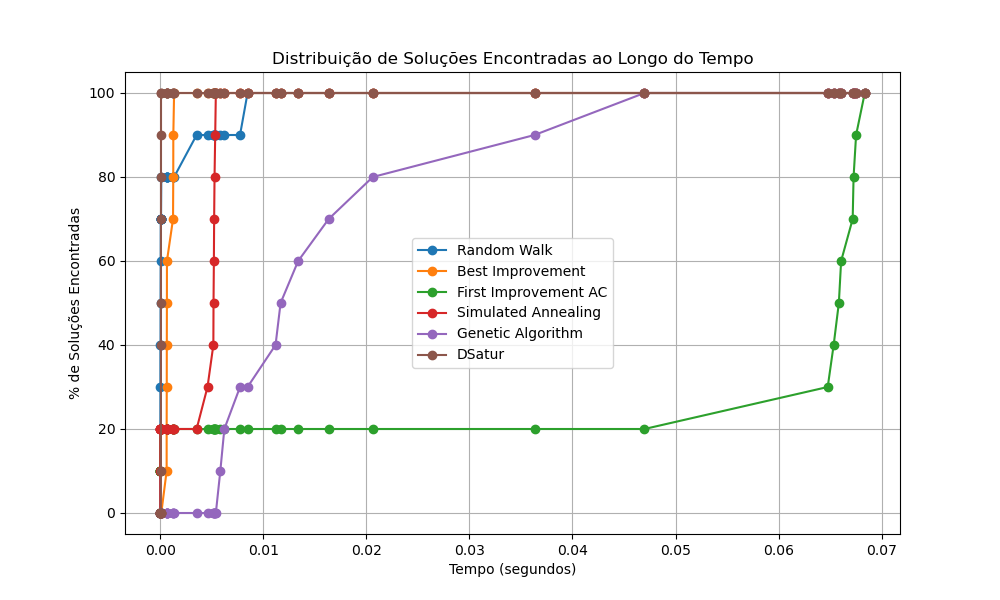
\includegraphics[width=1\textwidth]{./img/output-default.png}
    \caption{Experimento com a instância default.}
    \label{fig:experimento-default}
\end{figure}

Neste experimento, podemos observar que a heurística DSATUR se destacou significativamente, alcançando uma taxa de resolução de 100\% das instância quase instantaneamente, com um tempo médio de execução de apenas 0.01 segundos. Isso indica que o DSATUR é altamente eficiente para a instância default, conseguindo encontrar soluções ótimas rapidamente.


\begin{figure}[H]
    \centering
    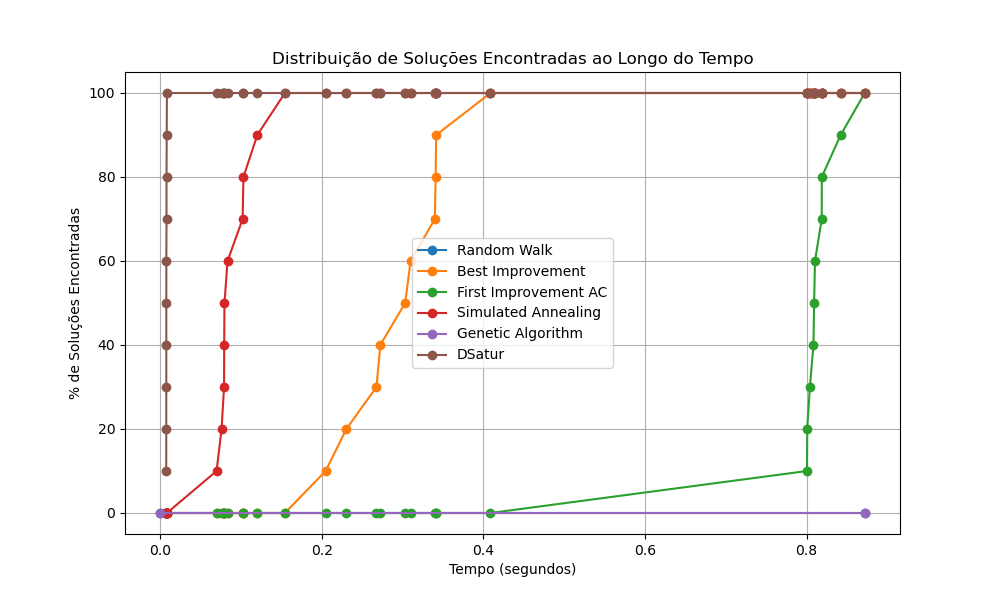
\includegraphics[width=1\textwidth]{./img/output-myciel5.png}
    \caption{Experimento com a instância myciel.5.col.}
    \label{fig:experimento-myciel5}
\end{figure}

\begin{figure}[H]
    \centering
    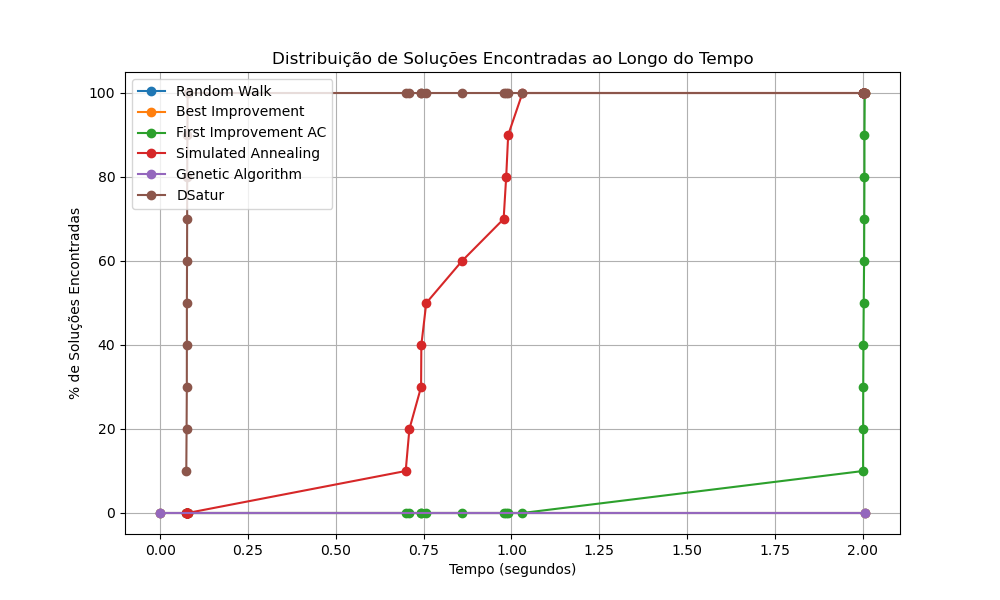
\includegraphics[width=1\textwidth]{./img/output-queen9-9.png}
    \caption{Experimento com a instância queen9-9.col.}
    \label{fig:experimento-queen9-9}
\end{figure}

Nos dois exeperimentos subsequentes, com as instâncias myciel.5.col e queen9-9.col, alguns algorítmos não encontraram soluções viáveis dentro do limite de tempo estabelecido. E por isto não aparecem nos gráficos. Esses resultados ressaltam a importância de considerar a complexidade do problema e a adequação das heurísticas utilizadas para diferentes instâncias.

Nos experimentos com instâncias maiores, como myciel.5.col e queen9-9.col, observamos que a heurística DSATUR continuou a se destacar, mantendo uma taxa de resolução de 100\% em ambas as instâncias. Isso demonstra a robustez e eficiência do DSATUR mesmo em problemas mais complexos.


\section{Conclusão}
Apresentar as conclusões gerais do trabalho, destacando os principais aprendizados e possíveis melhorias futuras.

\section*{Referências}
\bibliographystyle{plain}
Inserir todas as referências utilizadas no mesmo formato (ABNT, APA ou Vancouver).  
Exemplo em ABNT:
\bibliography{references}

\end{document}